\section{Results}\label{sec:results}


% \todo[inline]{I think we can summarize the following paragraphs for a few sentences}

In this section, we detail the findings of our study.  We remind the reader that our main goal with this study is to explore the
accuracy (false negative rate) of mining sandbox approaches using the corresponding state-of-the-art
test case generation tool (DroidBot), in the presence of a larger, representative dataset. We explore
the results of our research in our two datasets: the Small Dataset (101 pairs of apps) and the Complete Dataset (800 pairs of apps) as described in Section~\ref{sec:dataset}.

%%  and shed light on a few of
%% blindspots that impact the false negative rate. We hypothesize the presence of two blindspots - dynamic call trace from the entry point to a sensitive API, and the differences in the manifest file of repackaged apps. In Section~\ref{sec:Sensitive APIs}, we summarize the results of our study that estimates the performance of the state of the art in mining sandbox approaches. To this end, we reproduce the approach used by DroidBot in their original paper by presenting the divergent sensitive app sets for each app pair in our dataset. We also present details regarding which sensitive APIs are accessed more commonly with malwares. 
%% %We also present the 
%% %sensitive APIs set more injected by repackaged apps, among 162 explored. 
%% %We perform this initial study since it help solve our R1 and served as a reference to solve R2 and R3. \kn{How does this help solve R2 and R3.}

%% The remainder of this section is structured as follows. Section~\ref{sec:traceResults} presents the results of our study analyzing the impact of dynamic call trace on mining sandbox approaches, thereby answering R2. Section~\ref{sec:manifestResults} presents the results of our study analyzing the impact of modified manifest files on sandbox approaches, thereby answering R3. Section~\ref{sec:implications} presents some insights gained from the overall study and their potential implications.

\subsection{Small Dataset Assessment}

% \subsection{(Accuracy) False negative rate}\label{sec:Sensitive APIs}

In this section, we describe the results of reproducing the state-of-the-art Android sandbox approach, DroidBot on our small dataset of \num{101} pairs of apps.
Firstly, given a pair of apps, we analyse each app version using the DroidBot test case generation tool with the DroidXP infrastructure. We repeat
the dynamic analysis three times for a period of three minutes.

After the three executions, DroidXP produces a dataset with the sensitive methods that both app versions call during each execution. We consider that a test
generation tool, in our case, DroidBot, builds a sandbox able to detect a specific malware if there exists at least one call to a sensitive method that happens
only in the malicious version of the app. DroidXP also generates several reports, including the set of sensitive methods accessed by each app version (benign/malicious).
If the set of sensitive methods that only the malicious version of an app calls is empty,
we conclude that the sandbox approach for malware detection was not able to classify the malicious version as a malware, which leads to a false negative.

Considering the small dataset (101) apps, the mining sandbox approach for malware detection accurately classifies a total of \num{64} malware (\num{63.36}\%).
This result is similar when comparing it with the work of Bao et al., which reports a performance
of \num{66.66}\% for malware classification using
DroidBot~\cite{DBLP:conf/wcre/BaoLL18}

\subsubsection{Trace Analysis}

We then investigate if one could improve the performance of
the mining sandbox approach using a more elaborated comparison approach.
That is, instead of only comparing the sets of calls to sensitive APIs,
here we also compare the traces from entry points to such a calls.

Figure~\ref{fig:maliciousTrace} shows an example of a trace injected in the malicious version of the app \textbf{[com.android.remotecontrolppt]}.
Here, the benign and malicious app versions access the same sensitive method, \textit{getSubscriberid()}. This sensitive method returns the device's unique
subscriber ID, and requires the manifest file permission ``READ\underline{\space}PHONE\underline{\space}STATE'', present in both app versions.
The original app accesses this method through two distinct traces (Trace 01 and Trace 02), which suggests an expected action from app user. However,
instead of the 2 original traces, the malicious version injected a third trace (Trace 03) containing as entry point a method that performs a stealth
computation on a background thread, \textit{doInBackground}, suggesting an action without user's awareness.


\begin{figure}
\centering
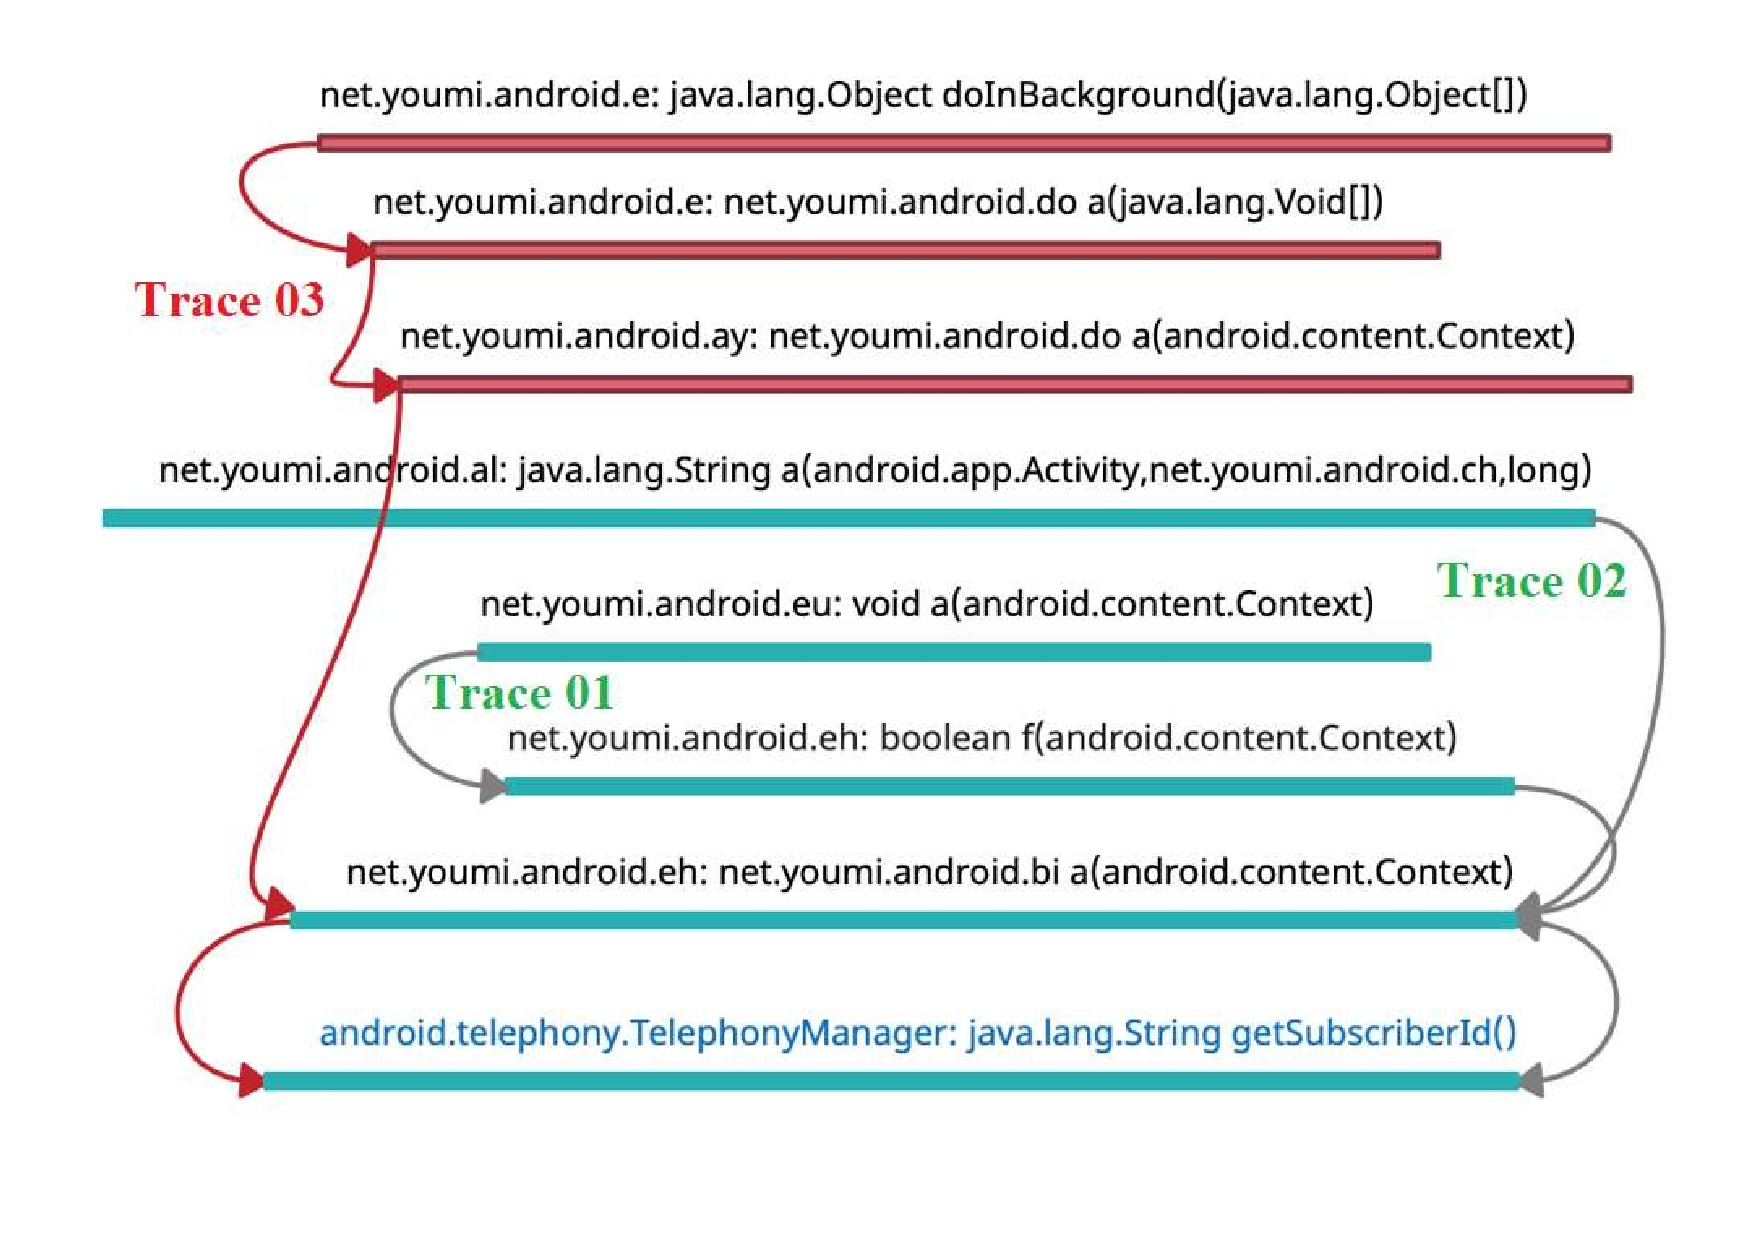
\includegraphics[scale=0.28]{images/maliciousTrace_example01.pdf}
\caption{Example of Malicious Trace.}
 \label{fig:maliciousTrace}
\end{figure}


In the small dataset, the vanilla mining sandbox approach fails
to detect \num{37} malware, using DroidBot as test case generator
tool. When we introduce trace analysis, we improve the
performance of the mining sandbox approach in \num{15.51}\%---
that is, using trace analysis, our approach correctly
classifies a total of 83 malware (\num{82.17}\% of the apps
in the small dataset). 

\begin{obs}{1}{}
  The use of Trace Analysis improves the performance
  of the mining sandbox approach to detect malware,
  from \num{66.66}\% to \num{82.17}\% in the
  Small Dataset. 
\end{obs}

\subsection{Manifest File Analysis}

Here we present the results of our investigation on the impact of modified Android Manifest files on the accuracy of sandbox approaches. This is
our second attempt for dealing with possible blindspots in the mining sandbox approach. 
To this end, we check some particular \emph{change patterns} in the manifest files, which might point out to automatic patches
that are necessary to include malicious behavior in repackaged apps. In section \ref{sec:manifestAnalysis}, we
illustrated that an automatic hacking script might inject permission requests within Android Manifest files regardless of whether this request is already present on it,
which can result in duplicated permissions and actions in these particular files.

We looked out for such modifications in the malware that went undetected by the
vanilla mining sandbox approach. In our small dataset set, out of the 37 repackaged apps the mining sandbox approach was not
able to correctly classify as malware, seven apps present duplicated permissions (DP), 12 apps present duplicated actions (DA), and
17 apps present either DP or DA. Table~\ref{tab:mfa} summarizes our results so far, where
VMS indicates the vanilla mining
sandbox approach, TA indicates the trace analysis, and MA indicates the manifest analysis.
Hits correspond to the total number of correctly identified malware using a given
combination of the proposed technique.

\begin{table}[ht]
  \centering
  \begin{small}
  \begin{tabular}{lcc}\toprule
  Technique      & Hits & Recall \\ \midrule 
  VMS            & 64   & \num{63.36}\% \\ 
  VMS + TA       & 83   & \num{82.17}\%  \\
  VMS + MA       & 81   & \num{80.19}\% \\
  VMS + TA + MA  & 91   & \num{90.09}\% \\  \bottomrule
  \end{tabular}
  \end{small}
    \caption{Summary of the results in the Small Dataset.}
 \label{tab:mfa}
\end{table}

\begin{obs}{2}{}
  The use of Manifest Analysis alone improves the performance
  of the mining sandbox approach to detect malware,
  from \num{66.66}\% to \num{80.19}\% in the
  Small Dataset. 
\end{obs}


It is to be noted that, when considering the small dataset, combining the manifest file analysis with the trace analysis
improves the accuracy rate to $90.09\%$, confirming that such an analysis, even though naive and simple,
does have an impact on the overall accuracy. Therefore, the Android manifest
analysis might also be used to complement the mining sandbox approach for malware detection.  


\begin{obs}{3}{}
  Combining Trace Analysis with Manifest Analysis improves the performance
  of the mining sandbox approach to detect malware,
  from \num{66.66}\% to \num{90.09}\% in the
  Small Dataset. 
\end{obs}

\subsection{Complete Dataset} 

Surprisingly, when applied to our complete dataset (\num{800} apps), the mining
sandbox approach correctly classifies only a total of \num{193} (\num{24.12}\%) malware---
for which the
repackaged version calls at least one additional sensitive API.
The accuracy of the approach here is much lower compared to what we reported for the
small dataset (previous section) as well as to what has been reported by previous works---e.g.,
Bao et al. (\num{66.66}\%)~\cite{DBLP:conf/wcre/BaoLL18} and Costa et al.
(\num{76.04}\%)~\cite{DBLP:journals/jss/CostaMMSSBNR22}. 
This indicates that when considering a more representative dataset, the accuracy of the mining sandbox
approach using DroidBot drops significantly. 

\begin{obs}{4}{}
  The mining sandbox approach for malware detection
  leads to a poor performance on the Complete Dataset (\num{800} pairs of apps),
  correctly classifying only \num{24.12}\% of the repackaged
  apps as malware in the complete dataset.
\end{obs}

We investigate whether or not the similarity between
the benign and malicious versions of every pair of apps
might explain this reduction on the performance of
the mining sandbox approach---using logistic regression.
The results suggest that we cannot explain the
poor performance of the mining sandbox approach
in terms of the difference between the overall similarity score that occurs in the
complete and small datasets. We also replicate this study using the
malware category feature, though we did not find
statistically significant evidence that the more representative
number of malware categories can explain the lower
performance of the mining sandbox approach in the
complete dataset. 


Therefore, DroidBot suffers from a significantly low accuracy rate when presented with a representative dataset, 
which encouraged us to endorse efforts aimed at identifying potential blindspots with such approaches.
Considering trace analysis, as we explained in Section~\ref{sec:pathsetup},
our results show that, among $607$ pairs of apps for which the vanilla mining
sandbox approach failed to classify the malicious version as malware, \num{176} of them ($29$\%) present different traces.
This result supports the hypothesis that the accuracy of the mining sandbox approach might be improved if the traces
from entry points to the calls to sensitive APIs are considered in the analysis.

Considering
manifest analysis, as we explained in Section~\ref{sec:manifestAnalysis},
looking at the occurrence of duplicated permissions and duplicated 
actions allows us to correctly classify \num{120} out of the \num{607} missed cases
from the mining sandbox approach (\num{19.76}\%).                                   
Table~\ref{tab:mfa-complete} summarizes the results of this investigation. When considering the 
complete dataset (\num{800} apps), combining the vanilla
mining sandbox approach (VMS) with trace analysis (TA) and
manifest analysis (MA) leads to the correct classification
of \num{446} malware (\num{55.75}\%), which suggests that
the mining sandbox approach requires further improvements when
we take into account a more representative dataset
of malware. 


\begin{table}[ht]
  \centering
  \begin{small}
  \begin{tabular}{lcc}\toprule
  Technique      & Hits & Recall \\ \midrule 
  VMS            & 193  & \num{24.12}\% \\ 
  VMS + TA       & 369  & \num{46.12}\%  \\
  VMS + MA       & 313  & \num{39.12}\% \\
  VMS + TA + MA  & 446  & \num{55.75}\% \\  \bottomrule
  \end{tabular}
  \end{small}
    \caption{Summary of the results in the Complete Dataset.}

 \label{tab:mfa-complete}
\end{table}

\begin{obs}{5}{}
  The results so far bring evidence that
  further research is necessary to understand
  the limitations of the mining sandbox approach
  targeting more comprehensive datasets.
\end{obs}

Our exploration of all sensitive APIs called by all app pairs brought to the light the most frequently abused sensitive APIs that
appear in the repackaged, malicious version of the apps. We observed that when executed all 800 app pairs, DroidBot called $75$ sensitive APIs at least one time (from our list of 162 sensitive APIs). Among them, $16$ APIs account for more than half of all calls ($51.06$\%).
%\rb{I could not understand the previous sentence}.
The sensitive API that is abused the most by repackaged apps is \textbf{android.telephony.TelephonyManager: java.lang.String getDeviceId()}, which gets the device
IMEI\footnote{From Wikipedia: International Mobile Equipment Identity (IMEI) is a number, usually unique, to identify 3GPP and iDEN mobile phones.}.
Table~\ref{tab:APIused} presents the list of the most frequent sensitive APIs that only the malicious
version of the apps in our dataset call.

\begin{obs}{5}{}
  The results so far bring evidence that only a handful of resources accesses like the \textbf{device id} are most attractive to malware designers, providing a potentially high-impact point of focus for future researchers and practitioners.
\end{obs}

%\begin{landscape}
\begin{table*}[t]
 \scriptsize
  \caption{Sensitive APIs more used by repackage apps}
  \centering
  %\begin{small}
 \begin{tabular}{lc}

   \toprule
   Sensitive API & Occurrences \\
   \midrule
   01 android.telephony.TelephonyManager: java.lang.String getDeviceId() &  78 \\
   02 android.net.wifi.WifiManager: android.net.wifi.WifiInfo getConnectionInfo() &  64\\
   03 android.net.wifi.WifiInfo: java.lang.String getMacAddress() &  63 \\
   04 android.net.NetworkInfo: java.lang.String getTypeName() &  58 \\
   05 android.net.NetworkInfo: java.lang.String getExtraInfo() &  56 \\
   06 android.telephony.TelephonyManager: java.lang.String getSubscriberId() &  54 \\
   07 android.net.NetworkInfo: android.net.NetworkInfo State getState() &  52 \\
   08 android.database.sqlite.SQLiteOpenHelper: android.database.sqlite.SQLiteDatabase getWritableDatabase() &  49 \\
   09 android.database.sqlite.SQLiteDatabase: android.database.Cursor query(java.lang.String, ...,java.lang.String) &  47 \\
   10 android.telephony.TelephonyManager: java.lang.String getNetworkOperator() &  45\\
   11 android.telephony.TelephonyManager: android.telephony.CellLocation getCellLocation() &  44\\
   12 android.database.sqlite.SQLiteOpenHelper: android.database.sqlite.SQLiteDatabase getReadableDatabase() &  44\\
   13 android.telephony.gsm.GsmCellLocation: int getLac() &  42 \\
   14 android.telephony.gsm.GsmCellLocation: int getCid() &  42 \\
   
   15 android.net.ConnectivityManager: android.net.NetworkInfo getNetworkInfo(int) &  39 \\
   16 android.telephony.TelephonyManager: java.lang.String getNetworkOperatorName() &  36 \\
   .&  .\\
   .&  .\\
   .&  .\\
   74 android.app.ActivityManager: java.util.List getRecentTasks(int,int) & 1 \\
   75 android.net.NetworkInfo: java.lang.String toString() & 1 \\

 \bottomrule
                            Total & 1592 \\

 \end{tabular}
 %\end{small}
 \label{tab:APIused}
\end{table*}
%\end{landscape}

%% \begin{obs}{1}{}
%%    %\kn{Here we need to add some final take aways of the reproduction study}
%%    Our results indicate that in the presence of a representative dataset ($800$ app pairs as opposed to $102$ and a diverse similarity index), the accuracy of state of the art in mining sandbox approaches, using DroidBot drops significantly (from $63.36\%$ to $24.12\%$). Our results also indicate that only few sensitive APIs are responsible for majority of injected malware in repackaged apps. This encourages the emergence of new proposals that can support mine sandbox mitigating \textit{blindspot}s that lead to low accuracy.
%%  \end{obs}


%\kn{In this subsection, are we simply reproducing the results of existing papers. Because as far as I understand, tools like DroidBOT etc. were evaluated by simply comparing the sensitive APIs call. I am guessing here our contribution is to evaluate it on the larger dataset. I have given it a shot, please keep me posted if this is correct.}

%% \subsection{Trace Analysis Results}\label{sec:traceResults}

%% In this section, we describe the results of our investigation on how the trace from the entry point to sensitive API could impact the accuracy of sandbox approaches. Initially, we collect the call graphs of DroidBot execution using \emph{Logcat} and filter in the traces between the app's entry point and calls to any sensitive methods.

%% Then, using the callgraph from executions of both app versions (benign/malicious), we track the differences between their traces. We choose to investigate only app pairs that covered the same set of sensitive APIs detected in both versions during our first experiment (Section~\ref{sec:Sensitive APIs}). 


%% \begin{obs}{2}{}
%%  The state of the art in mining sandbox approaches using DroidBot have a blind-spot when it comes to being aware of the trace taken from the entry point to a sensitive API call. The approaches could have a improvement of $22\%$ if it considered trace as a factor. Similar  improvements are also seen with the original dataset of $101$ app pairs (improvement of $18.81\%$).
%%  \end{obs}

%% \subsection{Manifest File Analysis}\label{sec:manifestResults}

%% In this section, we describe the results of our investigation on the impact of modified manifest files on the accuracy of sandbox approaches. 
%% To this end, we check some particulars from manifest file, that point to a likely suspicious behavior. In section \ref{sec:manifestAnalysis}, we illustrated that an automatic hacking script could inject permission requests at manifest file regardless of whether this request is already present on it, which can result in duplicated permission and actions in the Manifest file. We looked out for such modifications in the malware that went undetected by the test generation tools. Table~\ref{tab:mfa} summarizes our results.


%% The column (SAPI) indicates the number of malware that went undetected during our first study (same as Table~\ref{tab:pa}'s Same API set (SAPI)). The second column (DP) indicates how many Manifest files from malicious app undetected at first study, had duplicated permission. Same way, column (DA) denotes the number of Manifest files with the duplicated actions in their manifest file.

%% A duplicate request for permission or action in a malicious version's manifest file should have been performed by a script. A simple analysis of manifest file could detect $120$ of undetectable malware from the first experiment ($607$), if it considers explorer duplicate permissions or actions at manifest file code as a detection strategy. If we combine the previous trace analysis with manifest file analysis, we improve the accuracy rate to $55.75\%$.

%% It is to be noted that in the presence of the original dataset of $101$ app pairs, the manifest file analysis combined with the trace analysis earlier discussed improves the accuracy rate to $90.09\%$ confirming that such an analysis, even though naive and simple does have an impact on the accuracy rate of mining sandbox approaches.  %\kn{Handrick as before please put the full numbers in the table}


%% \begin{obs}{3}{}
%%  We can conclude that sandbox approach also could have better accuracy if they considered the suspicious modifications in manifest file in their analysis. Although the analysis required of the manifest file is quite naive, we believe the results present an interesting and relevant insight for developers of malware detection tools to improve accuracy.
%% \end{obs}

%% \todo[inline]{rb: I reviewed the paper until this point. I think that next we should
%% provide more explicit answers to the research questions. kn: Given this a shot}

%% \todo[inline]{mm: any finding we want to formulate related to the discussion in the last paragraph? kn: Given it a shot}

\section{Discussion}

In this section we elaborate on the answers to our research questions,
summarize the implications of our results, and discuss some possible
threats to the results we presented so far.

\subsection{Answers to the Research Questions}

The results we presented in the previous sections
give answers for our two research questions, as
we summarize in what follow.

\begin{enumerate}[(RQ1)]
  \item \textbf{\rqa} Although the accuracy rate of the state of the art in mining sandbox approaches was reported to be $66\%$ and later validated to be $63.26\%$ in our reproduction study in the presence of approximately $100$ app pairs, the accuracy rate drop to $24.12\%$ in the presence of more representative dataset of $800$ app pairs indicates that the \textcolor{blue}{accuracy of mining sandbox approaches does not scale}.

  \item \textbf{\rqb} Since the presence of a combination of trace and manifest analysis improved the accuracy by a factor of $23.34\%$ and $31.63\%$ to the accuracy of DroidBot in the presence of the small and complete dataset respectively, it is fair to say that \textcolor{blue}{the analysis of these two hypothesized blindspots do have a significant impact on the accuracy of mining sandbox approaches}. 
\end{enumerate}


\subsection{Implications}\label{sec:implications} 

Contrasting to previous research works~\cite{DBLP:conf/wcre/BaoLL18,DBLP:conf/iceccs/LeB0GL18,DBLP:journals/jss/CostaMMSSBNR22},
the results discussed in the previous sections lead to a more general understanding
about the limitations of using the Android mining sandbox approach
for malware detection. In particular, here we show that,
in the presence of a large dataset, the performance of the
approach drops significantly. Nonetheless, after running statistical tests (logistic regression),
we could not find evidence that the \emph{diversity} of the
complete dataset---in terms of similarity score and types of malware-could
justify the higher number of false negatives of the mining
sandbox approach. Therefore, further research is necessary to investigate
other possible reasons for that. Perhaps, the complete dataset
might contain a large percentage of malwares that use more
advanced techniques to evade from both static and dynamic analysis---
both methods are used in the mining sandbox approach
we discussed in this paper.

We also highlight that considering only the differences in the
sets of calls to sensitive APIs also leads to false negatives. We
argue in favor of using a more elaborate \emph{diff} approach, which
extends the mining sandbox approach to include the comparisons of
the dynamic call traces from the ``entry points'' of an Android app to its
set of calls to the sensitive APIs. We collect these call traces while
building the sandbox in the usual way~\cite{DBLP:conf/icse/JamrozikSZ16}. Using this extension, we could improve
the performance of the vanilla mining sandbox approach by a factor
between 19\% (small dataset) to 22\% (complete dataset). We
also explored a more ``complementary'' approach, somewhat independent
of the mining sandbox approach, which statically search for two
specific patterns of changes in the Android manifest files: permission
duplication and {\color{red}action duplication}. Using the manifest analysis,
we complement the performance of the mining sandbox approach, improving its performance by
a factor between 15\% (complete dataset) and 17\% (small dataset).
Altogether, the implications of this research are twofold:

\begin{description}
  \item[A warning to the community:] the mining sandbox approach for malware detection leads to a false negative rate higher than previous research reported. 
  \item[Future directions:] researchers should explore more advanced techniques for differentiating benign and malicious versions of the apps, while using the mining sandbox approach for malware detection. 
\end{description}  


